\onecolumn
\section{Vertices delivered across scales}
\label{app:cross-scale-witnesses}

We fix the first graph in each released test set (\texttt{idx\_0}) and retain all three benchmark seeds.
On small RB, both priority rules select the same 19 vertices at each seed. Resident OnlineMIS also
delivers 19 vertices each time, but shares only 5, 3 and 5 with SPRINT-C, respectively.
On large RB, the two priority rules each deliver 38 vertices at every seed, with 11, 34 and 22 in
common. On large ER, SPRINT-C delivers 371, 374 and 371 vertices, of which 17, 12 and 13 also
occur in the corresponding OnlineMIS sets. DIMES delivers 286 vertices at 109.2\,ms on the
third seed, its sole timely delivery on this graph. Of these, 29 also belong to the SPRINT-C set.
Full-cohort averages appear in Table~\ref{tab:external-deadline}.

\begin{figure}[!ht]
\centering
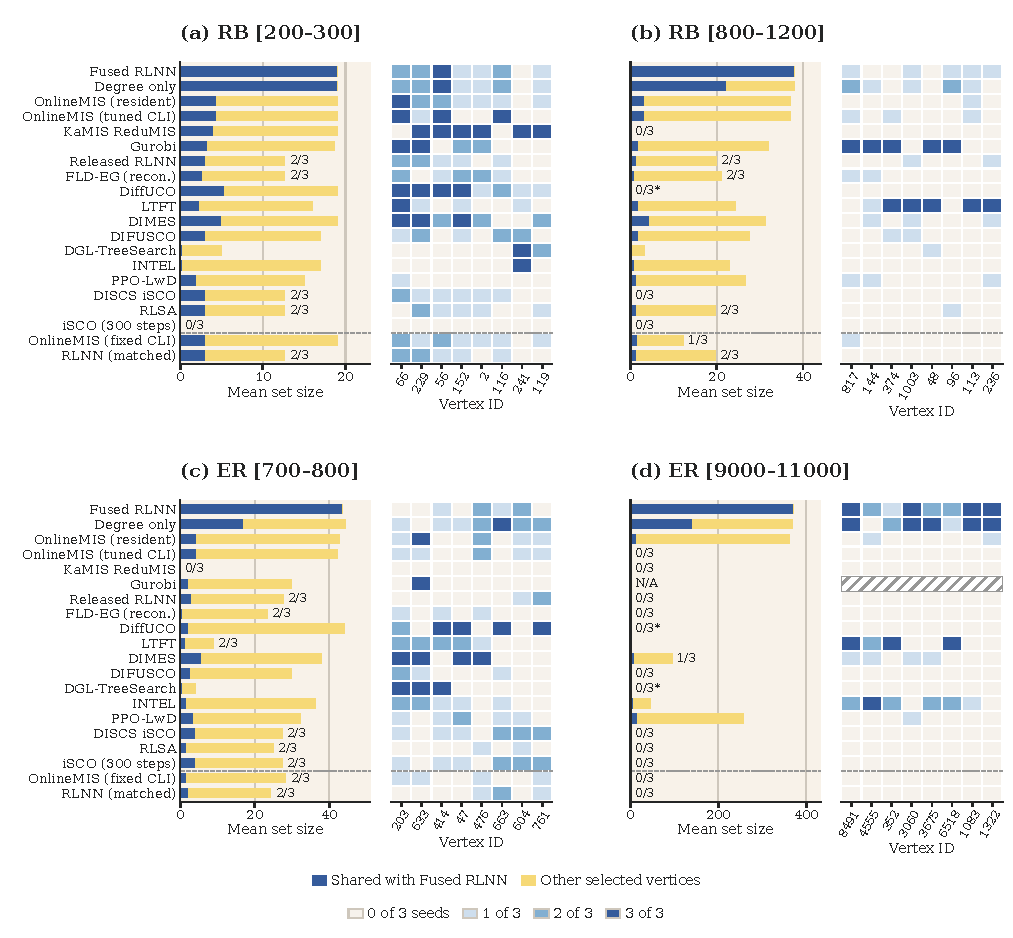
\includegraphics[width=\textwidth]{figures/cross_scale_witnesses.pdf}
\caption{\textbf{Four graphs, with vertex identities preserved across solvers and seeds.}
Each bar is the mean size of the set delivered by 200\,ms over seeds 1017, 1019 and 1021.
Blue counts vertices shared with SPRINT-C at the same seed and yellow counts the remaining
selected vertices. A fraction gives the number of timely deliveries when fewer than three
arrive. An asterisk marks a calibrated solver that skipped search because its predicted runtime
exceeded the budget. Hatching marks the large ER Gurobi model, which exceeds the installed
license limit. Each heatmap shows the eight vertices most frequently selected across the
main-table methods and seeds, ordered by frequency with ties broken by vertex ID. Cell shade
gives the number of seeds on which that solver delivered the vertex. The two rows below the
dashed line are the additional controls from Table~\ref{tab:scale-supplement}.}
\label{fig:cross-scale-witnesses}
\end{figure}
